\documentclass[12pt,titlepage]{extarticle}
% Document Layout and Font
\usepackage{subfiles}
\usepackage[margin=2cm, headheight=15pt]{geometry}
\usepackage{fancyhdr}
\usepackage{enumitem}	
\usepackage{wrapfig}
\usepackage{float}
\usepackage{multicol}

\usepackage[p,osf]{scholax}

\renewcommand*\contentsname{Table of Contents}
\renewcommand{\headrulewidth}{0pt}
\pagestyle{fancy}
\fancyhf{}
\fancyfoot[R]{$\thepage$}
\setlength{\parindent}{0cm}
\setlength{\headheight}{17pt}
\hfuzz=9pt

% Figures
\usepackage{svg}

% Utility Management
\usepackage{color}
\usepackage{colortbl}
\usepackage{xcolor}
\usepackage{xpatch}
\usepackage{xparse}

\definecolor{gBlue}{HTML}{7daea3}
\definecolor{gOrange}{HTML}{e78a4e}
\definecolor{gGreen}{HTML}{a9b665}
\definecolor{gPurple}{HTML}{d3869b}

\definecolor{links}{HTML}{1c73a5}
\definecolor{bar}{HTML}{584AA8}

% Math Packages
\usepackage{mathtools, amsmath, amsthm, thmtools, amssymb, physics}
\usepackage[scaled=1.075,ncf,vvarbb]{newtxmath}

\newcommand\B{\mathbb{C}}
\newcommand\C{\mathbb{C}}
\newcommand\R{\mathbb{R}}
\newcommand\Q{\mathbb{Q}}
\newcommand\N{\mathbb{N}}
\newcommand\Z{\mathbb{Z}}

\DeclareMathOperator{\lcm}{lcm}

% Probability Theory
\newcommand\Prob[1]{\mathbb{P}\qty(#1)}
\newcommand\Var[1]{\text{Var}\qty(#1)}
\newcommand\Exp[1]{\mathbb{E}\qty[#1]}

% Analysis
\newcommand\ball[1]{\B\qty(#1)}
\newcommand\conj[1]{\overline{#1}}
\DeclareMathOperator{\Arg}{Arg}
\DeclareMathOperator{\cis}{cis}

% Linear Algebra
\DeclareMathOperator{\dom}{dom}
\DeclareMathOperator{\range}{range}
\DeclareMathOperator{\spann}{span}
\DeclareMathOperator{\nullity}{nullity}

% TIKZ
\usepackage{tikz}
\usepackage{pgfplots}
\usetikzlibrary{arrows.meta}
\usetikzlibrary{math}
\usetikzlibrary{cd}

% Boxes and Theorems
\usepackage[most]{tcolorbox}
\tcbuselibrary{skins}
\tcbuselibrary{breakable}
\tcbuselibrary{theorems}

\newtheoremstyle{default}{0pt}{0pt}{}{}{\bfseries}{\normalfont.}{0.5em}{}
\theoremstyle{default}

\renewcommand*{\proofname}{\textit{\textbf{Proof.}}}
\renewcommand*{\qedsymbol}{$\blacksquare$}
\tcolorboxenvironment{proof}{
	breakable,
	coltitle = black,
	colback = white,
	frame hidden,
	boxrule = 0pt,
	boxsep = 0pt,
	borderline west={3pt}{0pt}{bar},
	% borderline west={3pt}{0pt}{gPurple},
	sharp corners = all,
	enhanced,
}

\newtheorem{theorem}{Theorem}[section]{\bfseries}{}
\tcolorboxenvironment{theorem}{
	breakable,
	enhanced,
	boxrule = 0pt,
	frame hidden,
	coltitle = black,
	colback = blue!7,
	% colback = gBlue!30,
	left = 0.5em,
	sharp corners = all,
}

\newtheorem{corollary}{Corollary}[section]{\bfseries}{}
\tcolorboxenvironment{corollary}{
	breakable,
	enhanced,
	boxrule = 0pt,
	frame hidden,
	coltitle = black,
	colback = white!0,
	left = 0.5em,
	sharp corners = all,
}

\newtheorem{lemma}{Lemma}[section]{\bfseries}{}
\tcolorboxenvironment{lemma}{
	breakable,
	enhanced,
	boxrule = 0pt,
	frame hidden,
	coltitle = black,
	colback = green!7,
	left = 0.5em,
	sharp corners = all,
}

\newtheorem{definition}{Definition}[section]{\bfseries}{}
\tcolorboxenvironment{definition}{
	breakable,
	coltitle = black,
	colback = white,
	frame hidden,
	boxsep = 0pt,
	boxrule = 0pt,
	borderline west = {3pt}{0pt}{orange},
	% borderline west = {3pt}{0pt}{gOrange},
	sharp corners = all,
	enhanced,
}

\newtheorem{example}{Example}[section]{\bfseries}{}
\tcolorboxenvironment{example}{
	% title = \textbf{Example},
	% detach title,
	% before upper = {\tcbtitle\quad},
	breakable,
	coltitle = black,
	colback = white,
	frame hidden,
	boxrule = 0pt,
	boxsep = 0pt,
	borderline west={3pt}{0pt}{green!70!black},
	% borderline west={3pt}{0pt}{gGreen},
	sharp corners = all,
	enhanced,
}

\newtheoremstyle{remark}{0pt}{4pt}{}{}{\bfseries\itshape}{\normalfont.}{0.5em}{}
\theoremstyle{remark}
\newtheorem*{remark}{Remark}


% TColorBoxes
\newtcolorbox{week}{
	colback = black,
	coltext = white,
	fontupper = {\large\bfseries},
	width = 1.2\paperwidth,
	size = fbox,
	halign upper = center,
	center
}

\newcommand{\banner}[2]{
    \pagebreak
    \begin{week}
   		\section*{#1}
    \end{week}
    \addcontentsline{toc}{section}{#1}
    \addtocounter{section}{1}
    \setcounter{subsection}{0}
}

% Hyperref
\usepackage{hyperref}
\hypersetup{
	colorlinks=true,
	linktoc=all,
	linkcolor=links,
	bookmarksopen=true
}

% Error Handling
\PackageWarningNoLine{ExtSizes}{It is better to use one of the extsizes 
                          classes,^^J if you can}


\def\homeworknumber{6}
\fancyhead[R]{\textbf{Math 140A: Homework \#\homeworknumber}}
\fancyhead[L]{Eli Griffiths}
\renewcommand{\headrulewidth}{1pt}
\setlength\parindent{0pt}


\DeclareMathOperator{\irr}{irr}

\begin{document}

\subsection*{29.6}

Note that

\[
    \alpha = \sqrt{3 - \sqrt{6}} \implies \alpha^2 - 3 = - \sqrt{6} \implies \alpha^4 - 6 \alpha^2 + 3 = 0
\]

meaning $\alpha$ is a zero of $f(x) = x^4 - 6x^2 + 3$ in $\Q[x]$. Since the Eisenstein criterion holds for $p = 3$, $f(x)$ is irreducible. Therefore $\irr(\alpha, \Q) = f(x)$ and $\deg(\alpha, \Q) = 4$

\subsection*{29.8}
Note that
\[
    \alpha = \sqrt{2} + i \implies \alpha^2 = 2 + 2 \sqrt{2} i - 1 \implies \alpha^4 - 2 \alpha^2 + 9 = 0
\]
meaning $\alpha$ is a zero of $f(x) = x^4 - 2x^2 + 9$ in $\Q[x]$. If $f$ was reducible over $\Q$, then it must have a zero in $\Z$ that divides 9. Checking $\pm 1, \pm 3$ gives no such zero, hence $f$ is irreducible. Therefore $\irr(\alpha, \Q) = f(x)$ and $\deg(\alpha, \Q) = 4$.

\subsection*{29.12}
Since $\pi \in \R$ then $\sqrt{\pi} \in \R$. Therefore it is algebraic in $\R$ with $\deg(\sqrt{\pi}, \R) = 1$ since it is a zero of the linear polynomial $f(x) = x - \sqrt{\pi}$.

\subsection*{29.16}
Since $(\pi^2)^3 - (\pi^3)^2 = 0$, then $\pi^2$ is a zero of the polynomial $f(x) = x^3 - \pi^6 \in \Q(\pi^3)$. This polynomial is irreducible hence $\pi^2$ is algebraic in $\Q(\pi^3)$ with $\deg(\pi^2, \Q(\pi^3)) = 3$.

\subsection*{29.18}
\subsubsection*{Part A}
\begin{proof}
    Note that
    \begin{align*}
        x = 0 &\implies 0^2 + 1 = 1 \neq 0 \\
        x = 1 &\implies 1^2 + 1 = 2 \neq 0 \\
        x = 2 &\implies 2^2 + 1 = 2 \neq 0
    \end{align*}
    Therefore $f(x)$ has no zero in $\Z_3$ and hence is irreducible.
\end{proof}

\subsubsection*{Part B}
\[
    \begin{array}{c|c|c|c|c|c|c|c|c|c}
        + & 0 & 1 & 2 & \alpha & 2 \alpha & 1+\alpha & 1+2 \alpha & 2+\alpha & 2+2 \alpha \\
        \hline 0 & 0 & 1 & 2 & \alpha & 2 \alpha & 1+\alpha & 1+2 \alpha & 2+\alpha & 2+2 \alpha \\
        \hline 1 & 1 & 2 & 0 & 1+\alpha & 1+2 \alpha & 2+\alpha & 2+2 \alpha & \alpha & 2 \alpha \\
        \hline 2 & 2 & 0 & 1 & 2+\alpha & 2+2 \alpha & \alpha & 2 \alpha & 1+\alpha & 1+2 \alpha \\
        \hline \alpha & \alpha & 1+\alpha & 2+\alpha & 2 \alpha & 0 & 1+2 \alpha & 1 & 2+2 \alpha & 2 \\
        \hline 2 \alpha & 2 \alpha & 1+2 \alpha & 2+2 \alpha & 0 & \alpha & 1 & 1+\alpha & 2 & 2+\alpha \\
        \hline 1+\alpha & 1+\alpha & 2+\alpha & \alpha & 1+2 \alpha & 1 & 2+2 \alpha & 2 & 2 \alpha & 0 \\
        \hline 1+2 \alpha & 1+2 \alpha & 2+2 \alpha & 2 \alpha & 1 & 1+\alpha & 2 & 2+\alpha & 0 & \alpha \\
        \hline 2+\alpha & 2+\alpha & \alpha & 1+\alpha & 2+2 \alpha & 2 & 2 \alpha & 0 & 1+2 \alpha & 1 \\
        \hline 2+2 \alpha & 2+2 \alpha & 2 \alpha & 1+2 \alpha & 2 & 2+\alpha & 0 & \alpha & 1 & 1+\alpha
    \end{array}
.\]
\vspace{5cm}
\[
    \begin{array}{c|c|c|c|c|c|c|c|c|c}
    \cdot & 0 & 1 & 2 & \alpha & 2 \alpha & 1+\alpha & 1+2 \alpha & 2+\alpha & 2+2 \alpha \\
    \hline 0 & 0 & 0 & 0 & 0 & 0 & 0 & 0 & 0 & 0 \\
    \hline 1 & 0 & 1 & 2 & \alpha & 2 \alpha & 1+\alpha & 1+2 \alpha & 2+\alpha & 2+2 \alpha \\
    \hline 2 & 0 & 2 & 1 & 2 \alpha & \alpha & 2+2 \alpha & 2+\alpha & 1+2 \alpha & 1+\alpha \\
    \hline \alpha & 0 & \alpha & 2 \alpha & 2 & 1 & 2+\alpha & 1+\alpha & 2+2 \alpha & 1+2 \alpha \\
    \hline 2 \alpha & 0 & 2 \alpha & \alpha & 1 & 2 & 1+2 \alpha & 2+2 \alpha & 1+\alpha & 2+\alpha \\
    \hline 1+\alpha & 0 & 1+\alpha & 2+2 \alpha & 2+\alpha & 1+2 \alpha & 2 \alpha & 2 & 1 & \alpha \\
    \hline 1+2 \alpha & 0 & 1+2 \alpha & 2+\alpha & 1+\alpha & 2+2 \alpha & 2 & \alpha & 2 \alpha & 1 \\
    \hline 2+\alpha & 0 & 2+\alpha & 1+2 \alpha & 2+2 \alpha & 1+\alpha & 1 & 2 \alpha & \alpha & 2 \\
    \hline 2+2 \alpha & 0 & 2+2 \alpha & 1+\alpha & 1+2 \alpha & 2+\alpha & \alpha & 1 & 2 & 2 \alpha
    \end{array}
.\]

\pagebreak

\subsection*{29.25}
\subsubsection*{Part A}
\begin{proof}
    Let $f(x) = x^3 + x^2 + 1$. Since $f(0) = 1$ and $f(-1) = 1$, $f$ has no zeroes in $\Z_2$ and is hence irreducible.
\end{proof}

\subsubsection*{Part B}
\begin{wrapfigure}[11]{l}{0.6\textwidth}
    \begin{center}
        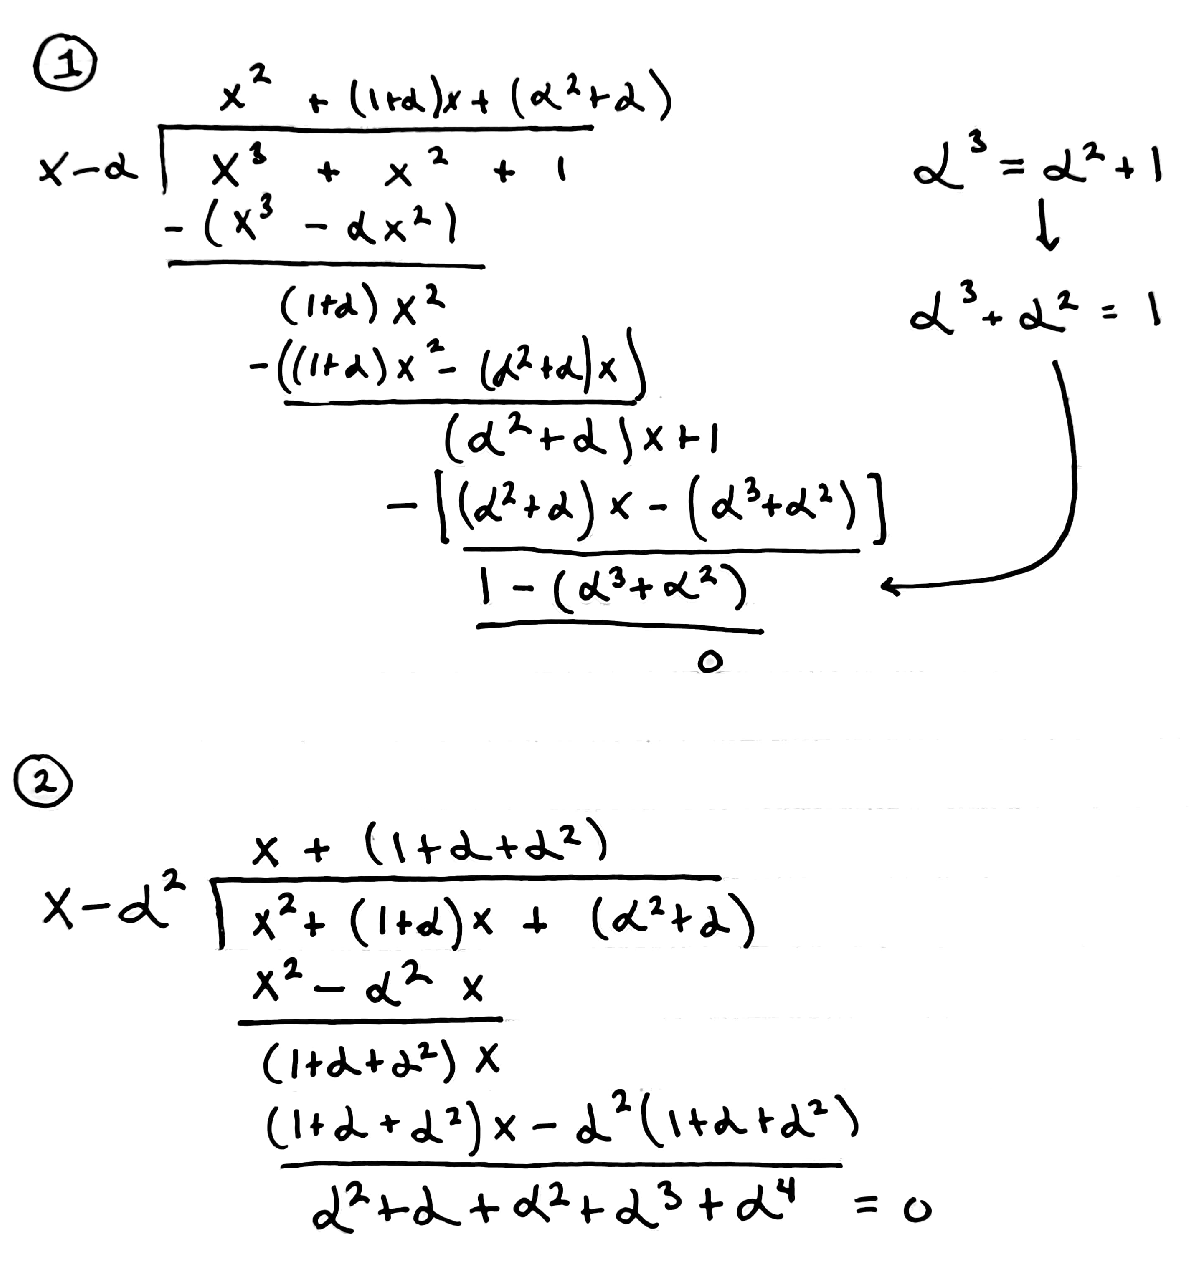
\includegraphics[page=1,width=0.5\textwidth]{longdiv2.pdf}
    \end{center}
\end{wrapfigure}

Part $(1)$ shows that $x - \alpha$ is a linear factor of $f(x)$. Checking $\alpha^2$ shows that is a zero of the remainder, hence doing another long division as demonstrated in $(2)$ gives another factor of $x - \alpha^2$. Therefore

\[
    x^3 + x^2 + 1 = (x - \alpha) (x - \alpha^2) (x + 1 + \alpha + \alpha^2)
.\]

in $\Z_2(\alpha)$.
\vspace{5cm}

\subsection*{29.26}
Since $\langle \Z_2(\alpha), + \rangle$ is abelian of order $8$ and $a + a = 0$ for all $a$ in it, it is isomorphic to just $\Z_2 \times \Z_2 \times \Z_2$. Furthermore, since $\langle \Z_2(\alpha), \cdot \rangle$ is abelian of order $7$, and $7$ is prime, then it must be isomorphic to just $\Z_7$.

\subsection*{29.29}
\begin{proof}
    Since $\alpha$ is algebraic in $F(\beta)$, there is a polynomial $f(x)$ with coefficients in $F(\beta)$ such that $f(\alpha) = 0$. The coefficients of $f$ have the form of a ration of two polynomials in $F[x]$. By mutliplying all the denominators together, a polynomial is achieved such that when multiplied with $f$, $f$ still remains $0$ but with coefficients in $\beta$. Since indeterminates are order-free, it follows $\beta$ is algebraic in $F(\beta)$
\end{proof}

\subsection*{29.30}
\begin{proof}
    Note that every element of $F(\alpha)$ can be expressed as
    \[
        b_0 + b_1 \alpha + \ldots + b_{n-1} \alpha^{n-1}
    .\]
    for $b_i \in F$. Since $F$ contains $q$ elements, there are $q$ choices for each coefficient that give each a unique element in $F(\alpha)$. Since there are $n$ coefficients, there are then $n$ choices meaning $q^n$ elements in $F(\alpha)$.
\end{proof}

\end{document}
